\documentclass[tikz,border=6pt]{standalone}

% общий стиль (подключается через TEXINPUTS)
% tikz-style.tex (общий стиль для всех TikZ-картинок)
\RequirePackage[T1,T2A]{fontenc}
\RequirePackage[utf8]{inputenc}

% Palatino-подобный шрифт (как в MathJax часто воспринимается «более вытянутым»)
\RequirePackage{txfonts}
% txfonts даёт предупреждение по кириллице (T2A/txr не определён).
% Оставляем txfonts для математики, а текстовый шрифт возвращаем на Computer Modern,
% чтобы не искать T2A/txr и убрать предупреждения.
\renewcommand{\rmdefault}{cmr}
\renewcommand{\sfdefault}{cmss}
\renewcommand{\ttdefault}{cmtt}

\RequirePackage{tikz}
\RequirePackage{xcolor}
\usetikzlibrary{calc}

% цвета
\definecolor{lightgreen}{RGB}{214,234,214}
\definecolor{darkgreen}{HTML}{0B7A0B}
\definecolor{darkred}{HTML}{DF0000}

\definecolor{midgreen}{HTML}{2E9B2E}
\definecolor{palegreen}{RGB}{235,246,235}
\definecolor{olivegreen}{HTML}{3E6B2F}

\definecolor{lightred}{RGB}{255,220,220}
\definecolor{midred}{HTML}{E04545}
\definecolor{darkred2}{HTML}{A80000}

\definecolor{lightblue}{RGB}{220,232,255}
\definecolor{midblue}{HTML}{2E5BD6}
\definecolor{darkblue}{HTML}{0B2E8A}

\definecolor{lightgray}{RGB}{240,240,240}
\definecolor{midgray}{RGB}{170,170,170}
\definecolor{darkgray}{RGB}{80,80,80}

\definecolor{vtxfill}{RGB}{86,193,255}
\definecolor{vennfill}{RGB}{220,232,255}


% единый набор стилей TikZ
\tikzset{
    lab/.style={
        font=\fontsize{24}{32}\selectfont
    }
}


\definecolor{vtxfill}{RGB}{86,193,255} % #56C1FF

\begin{document}
  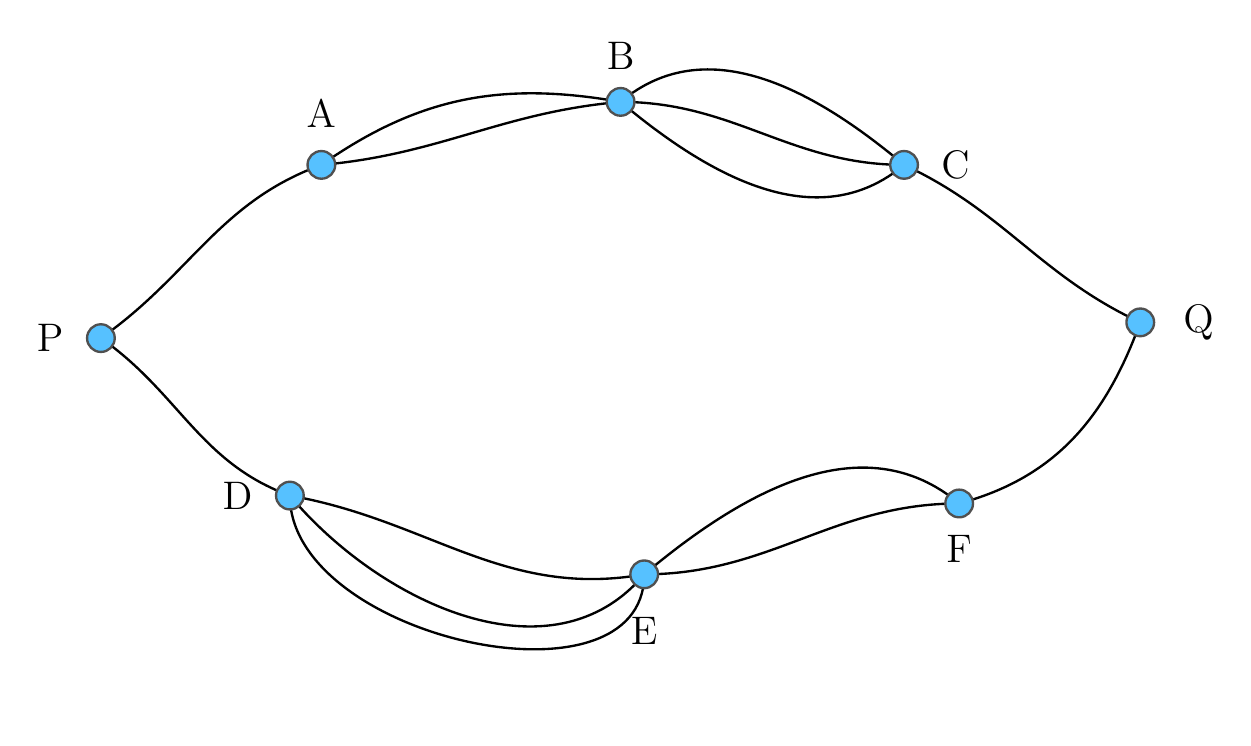
\begin{tikzpicture}[x=1cm,y=1cm, line cap=round, line join=round]

\tikzset{
  main/.style={draw=black, line width=0.85pt},
  vtx/.style={circle, draw=darkgray, fill=vtxfill, line width=0.85pt, minimum size=10pt, inner sep=0pt},
  vlab/.style={font=\Large},
}

% nodes
\coordinate (P) at (0,0);
\coordinate (A) at (2.8,2.2);
\coordinate (B) at (6.6,3.0);
\coordinate (C) at (10.2,2.2);
\coordinate (Q) at (13.2,0.2);
\coordinate (F) at (10.9,-2.1);
\coordinate (E) at (6.9,-3.0);
\coordinate (D) at (2.4,-2.0);

% edges P--A, P--D (outer)
\draw[main] (P) to[out=35,in=200] (A);
\draw[main] (P) to[out=-35,in=160] (D);

% edges A--B (upper arc + chord)
\draw[main] (A) to[out=35,in=170] (B);
\draw[main] (A) to[out=5,in=185] (B);

% edges B--C (three arcs, ~40° separation)
\draw[main] (B) to[out=40,in=140] (C);
\draw[main] (B) to[out=0,in=180] (C);
\draw[main] (B) to[out=-40,in=-140] (C);

% edge C--Q (outer)
\draw[main] (C) to[out=-25,in=155] (Q);

% edge Q--F (outer)
\draw[main] (Q) to[out=-110,in=15] (F);

% edges E--F (two arcs, ~40° separation)
\draw[main] (E) to[out=40,in=140] (F);
\draw[main] (E) to[out=0,in=180] (F);

% edges D--E (three arcs, ~40° separation)
\draw[main] (D) to[out=-10,in=-170] (E);
\draw[main] (D) to[out=-50,in=-130] (E);
\draw[main] (D) to[out=-90,in=-90] (E);

% vertices
\node[vtx] at (P) {};
\node[vtx] at (A) {};
\node[vtx] at (B) {};
\node[vtx] at (C) {};
\node[vtx] at (Q) {};
\node[vtx] at (F) {};
\node[vtx] at (E) {};
\node[vtx] at (D) {};

% labels
\node[vlab, left=10pt]  at (P) {P};
\node[vlab, above=10pt]  at (A) {A};
\node[vlab, above=8pt]  at (B) {B};
\node[vlab, right=10pt] at (C) {C};
\node[vlab, right=12pt] at (Q) {Q};
\node[vlab, below=8pt]  at (F) {F};
\node[vlab, below=12pt]  at (E) {E};
\node[vlab, left=10pt]  at (D) {D};

  \end{tikzpicture}
\end{document}